\subsection{Synchronous Agent interactions}
With the concepts introduced so far we can achieve already a lot in terms of agent interactions: agents can react to incoming events, which are either the \textit{Tick} event advancing simulation time by one step or a message sent by another agent (or the agent itself). This is enough to implement simple one-directional asynchronous agent interactions where one agent sends a message to another agent but does not await an answer within the same \textit{Tick}. This one-directional asynchronous interactions is used in the model to implement the passing of diseases, the paying back of debt, passing on wealth to children upon death - the agent simply sends a message and forgets about it.

Unfortunately this mechanism is not enough to implement the other agent-interactions in the Sugarscape model, which are structurally richer: they need to be synchronous. In the use-cases of mating, trading and lending two agents need to come to an agreement over multiple interactions steps within the same \textit{Tick} which need to be exclusive and synchronous.  This means that an agent A initiates such a multi-step conversation with another agent B by sending an initial message to which agent B has to react by a reply to agent A who upon reception of the message, will pick up computation from that point and reply with a new message and so on. Both agents must not interact with other agents during this conversation to guarantee resource constraints, otherwise it would become quite difficult and cumbersome to ensure that agents don't spend more than they have when trading with multiple other agents at the same time. Also the initiating agent A must be able to pick up processing of its \textit{Tick} event from the point where it started the conversation with agent B because sending a message always requires the handling of the current event to exit and hand the control back to the simulation kernel. See Figure \ref{fig:syncagentinteractions} for a visualisation of the sequence of actions.

\begin{figure}
	\centering
	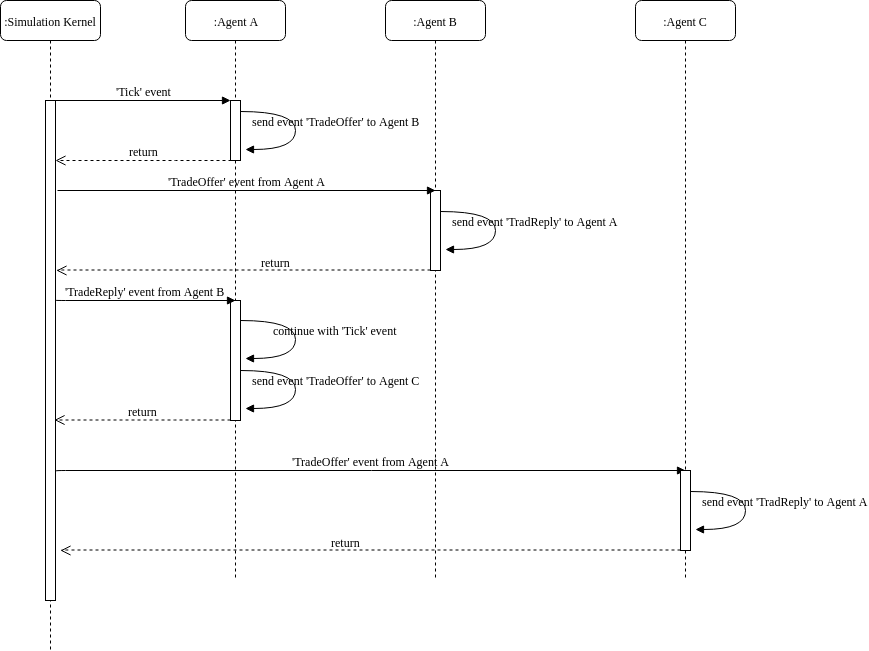
\includegraphics[width=1.0\textwidth, angle=0]{./fig/eventdriven/syncagentinteractions.png}
	\caption{Sequence diagram of synchronous agent interaction in the trading use-case. Upon the handling of the \textit{Tick} event, agent A looks for trading partners and finds agent B within its neighbourhood and sends a \textit{TradingOffer} message. Agent B replies to this message with \textit{TradeReply} and agent A continues with the trading algorithm by picking up where it has left the execution when sending the message to agent B. After agent A has finished the trading with agent B, it turns to agent C, where the same procedure follows.}
	\label{fig:syncagentinteractions}
\end{figure}

The way to implement this is to allow an agent to be able to change its internal event-handling state: to switch into different event-handlers, after having sent an event, to be able to react to the incoming reply in a specific way by encapsulating local state for the current synchronous interaction through closures and currying. Further, by making use of continuations the agent can pick up the processing of the \textit{Tick} event after the synchronous agent interaction has finished. Key to this is the function \textit{continueWithAfter} which we already shortly introduced through \textit{generalEventHandler}. This function takes an MSF which returns an output of type \textit{b} and an optional MSF. If this optional \textit{Maybe} MSF is \textit{Just} then the \textit{next} input is handled by this new MSF. In case no new MSF is returned (\textit{Nothing}), the MSF will stay the same. This is a more specialised version of the \textit{switch} combinator introduced in Chapter \ref{sec:back_frp} in the way that it doesn't need an additional function to produce the actual MSF continuation. Note that the semantics are different though: whereas \textit{switch} runs the new MSF immediately, \textit{continueWithAfter} only applies the new MSF in the \textit{next} step. The implementation of the function is as follows:

\begin{HaskellCode}
continueWithAfter :: Monad m => MSF m a (b, Maybe (MSF m a b)) -> MSF m a b
continueWithAfter msf = MSF (\a -> do
  ((b, msfCont), msf') <- unMSF msf a
  let msfNext = fromMaybe (continueWithAfter msf') msfCont
  return (b, msfNext))
\end{HaskellCode}

Finally, we can discuss the \textit{Tick} handling function. It returns a value of type \textit{Maybe (EventHandler g)} which if is \textit{Just} will result in to a change of the top-level event handler through \textit{continueWithAfter} as shown in \textit{generalEventHandler} above. Note the use of continuations in the case of \textit{agentMating, agentTrade} and  \textit{agentLoan}. All these functions return a \textit{Maybe (EventHandler g)} because all of them can potentially result in synchronous agent interactions which require to change the top-level event handler. The function \textit{agentDisease} is the last in the chain of agent behaviour, thus we are passing a default continuation which simply switches back into \textit{generalEventHandler} to finish the processing of a \textit{Tick} in an agent.

\begin{HaskellCode}
handleTick :: RandomGen g => DTime -> AgentLocalMonad g (Maybe (EventHandler g))
handleTick dt = do
  -- perform ageing of agent
  agentAgeing dt
  -- agent move, returns amount it of resources it harvested
  harvestAmount <- agentMove
  -- metabolise resources, depending on agents metabolism rate
  -- returns amount metabolised
  metabAmount <- agentMetabolism
  -- polute environment given harvest and metabolism amount
  agentPolute harvestAmount metabAmount

  -- check if agent has starved to death or died of age
  ifThenElseM
    (starvedToDeath `orM` dieOfAge)
    (do
      -- died of age or starved to deat: remove from simulation
      agentDies agentMsf
      return Nothing) 
    -- still alive, perform the remaining steps of the behaviour
    -- pass agentContAfterMating as continuation to pick up after mating
    -- synchronous conversations have finished
    (agentMating agentMsf agentContAfterMating)

-- after mating continue with cultural process and trading
agentContAfterMating :: RandomGen g => AgentLocalMonad g (Maybe (EventHandler g))
agentContAfterMating = do
    agentCultureProcess
    -- pass agentContAfterTrading as continuation to pick up after trading 
    -- synchronous conversations have finished
    agentTrade agentContAfterTrading 

-- after trading continue with lending and borrowing
agentContAfterTrading :: RandomGen g  => AgentLocalMonad g (Maybe (EventHandler g))
agentContAfterTrading = agentLoan agentContAfterLoan

-- after lending continue with diseases, which is the step in a Tick event
agentContAfterLoan :: RandomGen g => AgentLocalMonad g (Maybe (EventHandler g))
agentContAfterLoan = agentDisease defaultCont

-- safter diseases imply switch back into the general event handler
defaultCont :: RandomGen g => AgentLocalMonad g (Maybe (EventHandler g))
defaultCont = return (Just generalEventHandler)
\end{HaskellCode}

\subsubsection{Synchronous through Tagless Final}
TODO: the indirect, continuation based approach is cumbersome and it is easy to get something wrong, thus synchronous interactions would be desirable. With the tagless final approach as introduced in the TODO section, this becomes possible
TODO: show the syncSend approach of SIR and discuss the problem of not being able to recursively send to itself e.g. agent A initiates syncSend, then it cannot send directly to itself or if it sends to agent B this agent B cannot send another syncSend to agent A. Or A -> B -> C -> A is also not possible, any chain which comes back to the originator leads to wrong semantics where effects might be visible but the changes to the last agent will be overridden.

further ideas for tagless final in sugarscape:
- all creation and removal related stuff create new agent does not require id but kernel returns new id